\documentclass{article}
\pdfpagewidth 8.5in
\pdfpageheight 11in 

\setlength\topmargin{0in}
\setlength\headheight{0in}
\setlength\headsep{0in}
\setlength\textheight{7.7in}
\setlength\textwidth{6.5in}
\setlength\oddsidemargin{0in}
\setlength\evensidemargin{0in}
\setlength\parindent{0.25in}
\title{ZK Failover Controller Design}
\author{Todd Lipcon\\todd@cloudera.com}
\usepackage{hyperref}
\usepackage{graphicx}
\usepackage{graphviz}
\usepackage{verbatim}
\begin{document}
\maketitle
\tableofcontents

\section{Overview}

\subsection{Background}
HDFS-1623 and related JIRAs added high availability support to the HDFS NameNode,
but rely on an administrator to manually trigger the failover process. As per
the original design doc, manual failover addresses many of the scenarios in which
cluster downtime was previously unavoidable; for example, the administrator
may now upgrade or replace hardware or software on one NameNode machine
after failing over to the standby, without any loss of availability.

However, HDFS-1623 did not address {\em automatic} failover. By contrast,
automatic failover relies on a failure detector to automatically decide that the
active NameNode has become unavailable and trigger a fail-over to the warm standby.

\subsection{ZooKeeper-based approach}

This document describes the design for a method of automatic failover based on
Apache ZooKeeper. ZooKeeper (henceforth ``ZK'') is itself highly available and
provides the following features upon which we can build:
\begin{itemize}
\item A strongly consistent repository for small amounts of arbitrary information ({\em znodes})
\item The ability to create a znode which is automatically deleted when the creator's client fails (an {\em ephemeral} node.
\item The ability to monitor and be asynchronously notified when the state of a znode changes. ({\em watchers})
\end{itemize}

Using the above features, this design uses ZooKeeper in several key ways:
\begin{itemize}
\item {\bf Failure detector} - the active NameNode creates an ephemeral node in ZK. If the active should fail, the ephemeral node will be automatically deleted after a configurable timeout.
\item {\bf Active node locator} - by writing a small amount of information into ZK, clients or other services can locate the current active node authoritatively
\item {\bf Mutual exclusion of active state} - since ZK is consistent and highly available, we can use it to ensure that at most one node is active at any time.
\end{itemize}

Other designs for automatic failover could substitute different components for some or all of the above. For example, the Linux-HA project can provide some of the same building blocks. Nevertheless, ZK is particularly attractive because it satisfies all aspects in a single system, with no external configuration. Many Hadoop deployments also already deploy ZooKeeper for other applications such as Apache HBase.

\section{Design}

\subsection{Components} 
The design for ZK-based automatic failover consists of three main components:
\begin{enumerate}
\item A {\tt HealthMonitor} implementation, which watches a NameNode to see if the process has become unavailable or entered an unhealthy state
\item A {\tt ActiveStandbyElector} implementation, which manages and monitors state in ZooKeeper
\item A {\tt ZKFailoverController} implementation, which subscribes to events from {\tt HealthMonitor} and {\tt ActiveStandbyElector}, and manages the state of the NameNode. The ZKFC also takes care of fencing the prior NameNode if it enters an indeterminate state.
\end{enumerate}

In the current design, all three of the above components run in the same JVM. This JVM runs on the same host as the NameNode, but is distinct from the NameNode itself. We'll call the JVM as a whole the {\em ZKFC process}. Thus, in a typical HA cluster with two NameNodes, each NameNode machine runs its own ZKFC process.

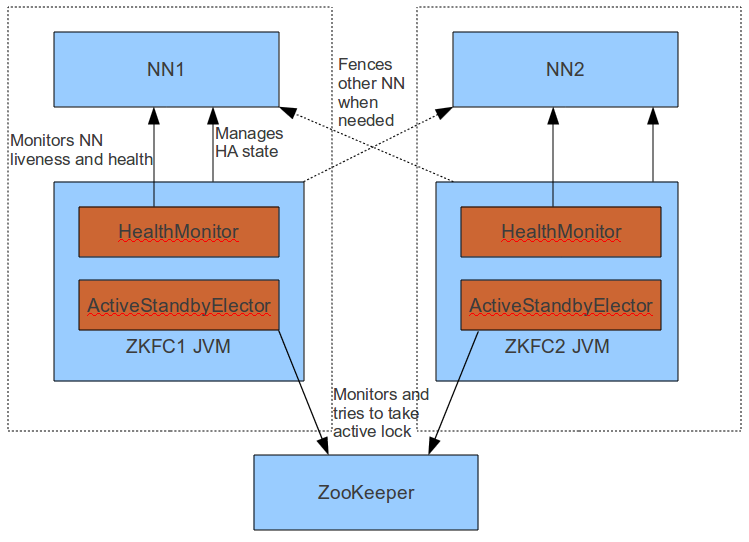
\includegraphics[width=6in]{components.png}

\subsection{HealthMonitor design}

The HealthMonitor (committed in HADOOP-7788) is a thread which is responsible for monitoring the local NameNode. It operates in a simple loop, calling the {{monitorHealth}} RPC. The HealthMonitor maintains a view of the current state of the NameNode based on the responses to these RPCs. When it transitions between states, it sends a message via a callback interface to the ZKFC. It has the following states:

\begin{itemize}
\item {\bf \tt INITIALIZING} - The HealthMonitor is starting up and has not yet contacted the NN
\item {\bf \tt SERVICE\_NOT\_RESPONDING} - The health check RPCs are timing out or otherwise not returning either a definitive success or failure
\item {\bf \tt SERVICE\_HEALTHY} - the health check RPCs are returning success
\item {\bf \tt SERVICE\_UNHEALTHY} - the health check RPCs are returning a definitive failure (eg the NameNode has itself detected some health issue like being out of local disk space)
\item {\bf \tt HEALTH\_MONITOR\_FAILED} - the health monitor thread has crashed due to an uncaught exception, etc. This is generally a fatal error causing an abort.
\end{itemize}

\subsection{ActiveStandbyElector design}

The ActiveStandbyElector (committed in HADOOP-7992 and improved in HADOOP-8163, HADOOP-8212) is responsible for coordinating with ZooKeeper. The ZKFC interacts with it mainly by two main calls:
\begin{itemize}
\item {\tt joinElection(...)} - indicate to the ASE that the local NameNode is a candidate to become active.
\item {\tt quitElection(...)} - indicate to the ASE that the local NameNode is no longer a candidate to become active (e.g because its health has gone bad)
\end{itemize}

After the ZKFC calls {{joinElection}}, the ASE will attempt to acquire a lock in a configurable location in ZooKeeper. This lock consists of an ephemeral znode, such that it will automatically be deleted should the ZKFC process crash, or the node lose its network connection. If the ASE successfully creates the lock, then it will call {\tt becomeActive()} on the ZKFC. Otherwise, it calls {\tt becomeStandby()} and begins to monitor the other node's lock.

In the case that the current lock holder fails, another ZKFC's watch on that node will trigger, causing it to attempt to grab the lock. If it succeeds, the ASE will indicate to the ZKFC that it should now become active with the same {\tt becomeActive()} call.

In the event that the ZooKeeper session expires, the ASE will call {\tt enterNeutralMode} on the local node. It does not, however, call {\tt becomeStandby}, since it has no way of knowing whether another node is ready to take over. The transition of the local node to Standby in this case is handled by the fencing mechanisms (see below).

\subsection{ZKFC Design}

The ZKFC is itself relatively simple. It runs the following process:

\begin{itemize}
\item On startup, initialize the HealthMonitor to monitor the local NameNode. Initialize the ActiveStandbyElector with the configured ZooKeeper quorum information. Do {\em not} immediately try to join the election.
\item When the HealthMonitor's state changes, respond as follows:
  \begin{itemize}
  \item {\tt SERVICE\_HEALTHY} - instruct the elector to join the election if not yet joined
  \item {\tt HEALTH\_MONITOR\_FAILED} - abort the whole ZKFC process, since it can no longer function as designed
  \item {\tt INITIALIZING} - in this case, the local node has just restarted, and not ready to service calls. Quits the election, and indicates that fencing is unnecessary, since the NameNode always starts in Standby state.
  \item Other states - quit the election if currently in the election
  \end{itemize}
\item When the ActiveStandbyElector instructs a change, respond as follows:
  \begin{itemize}
  \item {\tt becomeActive()} - call {\tt transitionToActive()} on the local node. If it fails, quit the election.
  \item {\tt becomeStandby()} - call {\tt transitionToStandby()} on the local node. If it fails, then the other node will be fencing this node anyway. (see below)
  \item {\tt enterNeutralMode()} - currently no response, as there is no such state in the current HA design
  \item {\tt fenceOldActive(...)} - see below
  \item {\tt notifyFatalError(...)} - abort the ZKFC process, since it is no longer functioning as expected
  \end{itemize}
\end{itemize}

All of the calls are synchronized on the ZKFC object, such that there is a clearly serialized order of events impacting its logic.

\subsection{Fencing}

HADOOP-8163 enhanced the ActiveStandbyElector design to provide hooks for fencing. The enhancement was as follows:
\begin{enumerate}
\item After obtaining the active lock, but before instructing the local process to become active, check for the presence of a {\em breadcrumb} znode.
  \begin{enumerate}
  \item If it exists, call {\tt fenceOldActive(data)} passing the data from that node. If fencing is successful, delete the breadcrumb node.
  \item If fencing fails, log an error, drop the lock, sleep, and rejoin the election. This gives other nodes a chance to try to fence.
  \item Create a new breadcrumb node with the local node's identifying data
  \end{enumerate}
\item When quitting the election, allow the quitting node to specify whether it may need fencing. If it does not need fencing, delete the breadcrumb node before closing the ZooKeeper session.
\end{enumerate}

\subsection{ZKFC State machine diagram}

\includedot[scale=0.5]{state-machine}


\section{Example scenarios}

\subsection{Active NN JVM crash}

When the JVM crashes, the HealthMonitor on the same node will fail its {\tt monitorHealth()} call, due to a timeout or a connection-refused error. The HM then triggers {\tt enterState(SERVICE\_NOT\_RESPONDING)} to the ZKFC. The ZKFC quits the election. The ZKFC on the other node successfully obtains the active lock, initiates fencing, and becomes active.

\subsection{Active NN JVM freeze (e.g SIGSTOP)}

If the ANN's JVM freezes, but does not crash, the scenario is the same as above. The {\tt monitorHealth()} call will hit an RPC timeout and trigger failover.

{\bf Future work:} using JVMTI we may be able to determine externally whether the NN JVM is currently experiencing a lengthy garbage collection pause. We could then use a different timeout for failover due to GC pauses.

\subsection{Active NN machine crash}

When the whole machine crashes, the ActiveStandbyElector will lose its lease in ZooKeeper after the configured session timeout. The other node's ZKFC will notice the deletion of the lock, and proceed the same as above to trigger failover.

\subsection{Active NN goes unhealthy}

When the health state changes, the HealthMonitor will see a {\tt HealthCheckFailedException} and trigger failover the same as above.

\subsection{Active ZKFC crashes}

The ZKFC runs in a separate process which is designed to be very simple. However, it is still possible for it to crash (e.g due to a JVM bug, bad memory, etc). In this case, failover will be falsely triggered. Before using aggressive fencing, the failover controller on the other node will issue a {\tt transitionToStandby} to the original node to gracefully give up its active state. This will succeed, since the NameNode itself is healthy. Thus, an unnecessary failover is triggered, but the system proceeds as expected.

\subsection{ZooKeeper crash}

If ZooKeeper itself crashes, then both ZKFCs will receive a {\tt DISCONNECTED} event at the same time. Upon this event, they call {\tt enterNeutralMode} on the local NameNode, but neither makes any change in state. Thus, the system keeps running while ZooKeeper is down -- it is just unable to perform a failover.

When ZooKeeper returns, the clients will immediately reconnect. ZooKeeper's behavior is such that client sessions that were present before the crash are allowed to re-acquire their session so long as they reconnect within their session timeout, starting at the time of restart\footnote{See \url{https://cwiki.apache.org/confluence/display/ZOOKEEPER/FAQ}, confirmed by phunt}. So, both nodes will regain their session correctly and no unnecessary failovers will be triggered.

{\bf Future work:} the breadcrumb znode could be used in this circumstance to give preference to the node that was active before the ZK outage.

\section{Details yet to be ironed out}

\subsection{Integrating manual failover}
Even with automatic failover in place, an administrator may want to trigger manual failover for some other reason (e.g. a hardware upgrade on the active node). Currently, the design does not take administrative input. As a workaround in the initial implementation, the administrator can simply shut down the active NameNode using the usual service management infrastructure. This will initiate a failover within a small number of seconds.

This can be improved by adding a simple RPC interface to the ZKFC which provides an {\tt quiesceActiveState()} call. This call would instruct the NN to leave the election and wait several seconds for the standby node to trigger the failover. If no failover occurs within several seconds, it can re-obtain the active lock and report an error to the administrator.

\section{Future work}

\subsection{Preferential nodes}
In some deployments, the adminsitrator may prefer to mark one of their multiple NameNodes as the preferred active. The current design does not allow for that: when the failover controllers start up, they race to take the active lock, and whoever wins the race becomes active. We may want to provide the ability to delay joining the election on the non-preferred node, or even to automatically trigger failback from the non-preferred to the preferred node, even when the non-preferred node remains healthy.

\subsection{Self-fencing}

When the HM indicates that the local node has gone unhealthy, the ZKFC could initiate a self-fencing step before quitting the election. For example, it can use {\tt fuser -k -9 <ipcport>} to forcefully kill the local NameNode. With this in place, it can avoid many scenarios in which more expensive/complicated fencing mechanisms would otherwise be tried.

\subsection{Process supervision}
The current design supposes that the ZKFC process and the NameNode process are run independently by service scripts or a cluster management framework. In the event that the NameNode crashes, the ZKFC makes no attempt to re-start it. Instead, it simply ocntinues to monitor the IPC port until the NameNode is restarted by some other means. We assume that existing cluster monitoring is in place to notify the cluster operator, who will take action to restart the NN.

Instead, one could imagine the ZKFC process actually starting (and restarting) the NN. This could make deployment simpler, though it has the downside of adding some complexity to the ZKFC itself, since process management in Java can be messy. Nevertheless, the current design is modular enough that adding this facility would be a  straightforward extension of the current work.

\section{Test plan}

TBD

\section{Revision history}

\verbatiminput{|"git log"}
\end{document}
